\documentclass{jsarticle}

\usepackage{amsmath,amssymb}
\usepackage{bm}
\usepackage{braket}
\usepackage[dvipdfmx]{graphicx}
\usepackage{here}

\begin{document}
\part{BdGモデルハミルトニアンについて}
	\section{定義}
		BdGモデルハミルトニアン$\mathcal{H}$は以下のように表される。

		\begin{align}
			\mathcal{H}=\int \vec{\Psi}^\dagger \tilde{H}\vec{\Psi}dr
		\end{align}

		\begin{align}
			\int dr=\int dxdy
		\end{align}

		\begin{align}
			\vec{\Psi}=
			\begin{bmatrix}
				\Psi_\uparrow \\
				\Psi_\downarrow \\
				\Psi_\uparrow^\dagger \\
				\Psi_\downarrow^\dagger
			\end{bmatrix}
		\end{align}

		\begin{align}
			\tilde{H}=
			\begin{bmatrix}
				\hat{h}(r) & \hat{\Delta}(r) \\
				-\hat{\Delta}^\ast(r) & -\hat{h}^\ast(r)
			\end{bmatrix}
		\end{align}

		\begin{align}
			\hat{h}=\left[-\frac{\hbar^2}{2m}\nabla^2-\mu_F \right]\hat{\sigma}_0 \\
			\left( \hat{\sigma}_0:単位行列 \right)
		\end{align}

		\begin{align}
			\hat{\Delta}(r)=
			\begin{cases}
				\Delta_0 \left( i \hat{\sigma}_2 \right) & \mbox{s-wave} \\
				\Delta_0\frac{i\partial x}{k_F}\hat{\sigma}_1 & \mbox{ $p_x$-wave} \\
				\Delta_0\frac{1}{k_f} \left( \hat{\sigma}_1+i\hat{\sigma}_2 \right) & \mbox{$p_x+ip_y$}
			\end{cases}
			\label{Delta}
		\end{align}

		\begin{align}
			\vec{\Psi}=\frac{1}{\sqrt{Ly}}\sum_{k_y} \vec{\Psi}_{k_y}(x) e^{ik_yy}
		\end{align}

		\begin{figure}[H]
			\centering
			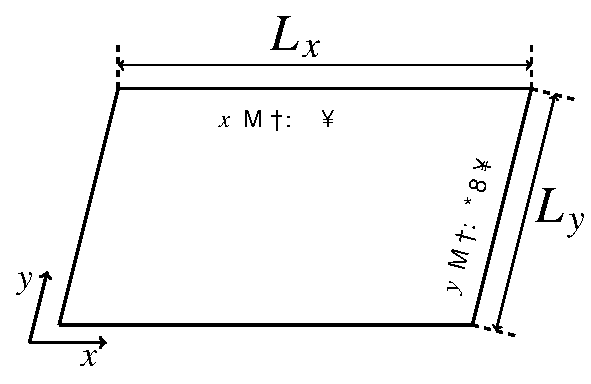
\includegraphics[scale=1]{figure1}
			\caption{考える系}
			\label{system}
		\end{figure}
\end{document}
